\section{Classification}
%Report on performances when running the different classifiers. Report on values tested for i) the hyperparameters, ii) the training/testing ratios, iii) number of folds for crossvalidation. Give performance results only for the most interesting choices of hyperparameters, training/testing ratios and number of folds.

In this section, we will quantify the performance of different methods of classification in a quantitative manner using the F-measure. We will also compare the sensitivity of the algorithm's performance regarding to the choice of hyper-parameters and the splitting ratio between training and testing set. 

\subsection{GMM}
GMM and Bayes technique depends on different hyper-parameters such as the covariance matrix or the number of components per class. We will evaluate quantitatively the impact of each parameters on the performance and we will compare the F-measure for a set of parameters to tackle the issue of over-fitting. 

Firstly, we have evaluated the effect of number fold in the cross-validation. In \texttt{MLDEMOS}, the number of fold seems to be the number of times we trained the model. In fact, we can tune the training/test ratio and we can see that with a low number of folds such as 2, the F1-measure is not representative. But with a number of folds of 10, the results are coherent. We decided to keep a 10-fold for the following.  

Secondly, we have evaluated the effect of the training/testing ratio on the performance. We kept the same parameter to compare the performance. We set a full covariance matrix with 1 component per class. Results are shown in figure \ref{fig:train_ratio}


\begin{figure} [ht]
\centering
	\begin{subfigure}[h]{0.32\textwidth}
    \centering
	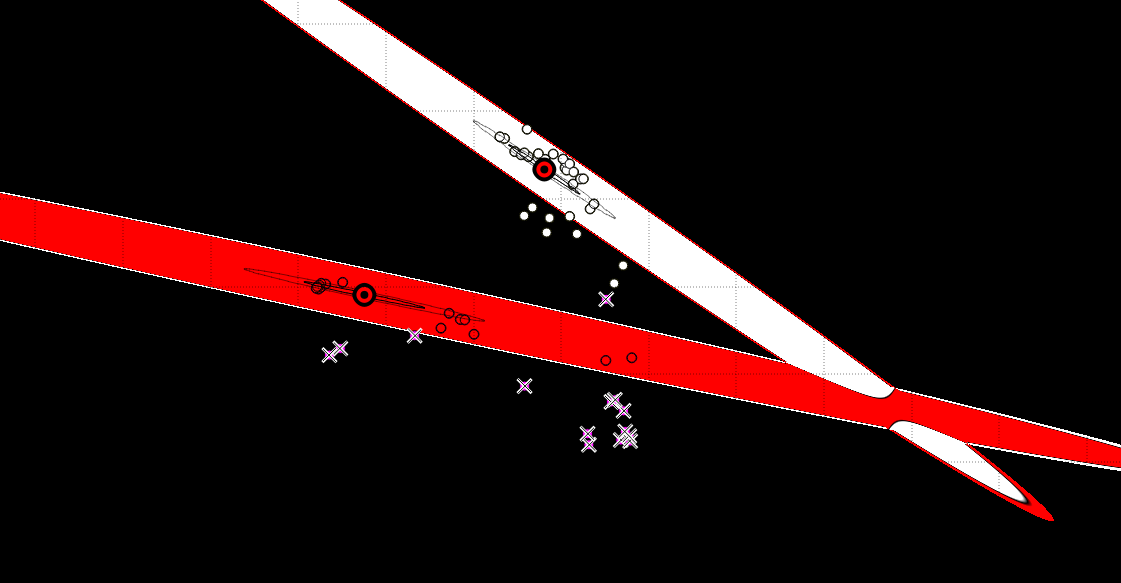
\includegraphics[height=0.11\textheight]{./classification/full_var_gmm_1_10pourcent_test.png}
	\caption{\bf Train ratio = 10\%}
	\end{subfigure}
    \begin{subfigure}[h]{0.32\textwidth}
    \centering
    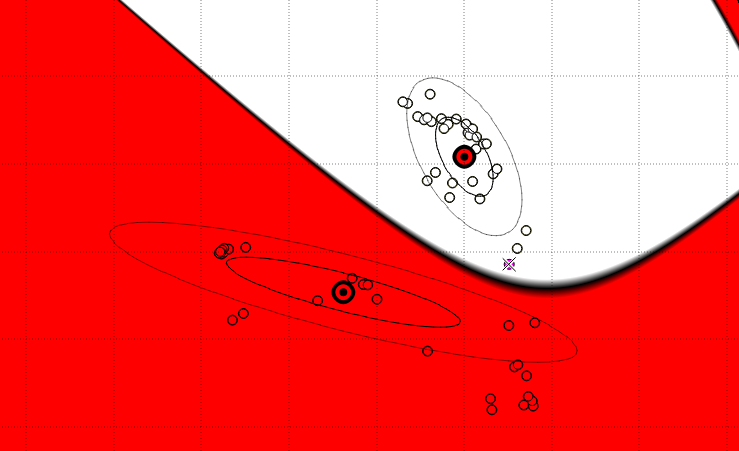
\includegraphics[height=0.11\textheight]{./classification/full_var_gmm_1_50pourcent_test.png}
	\caption{\bf Train ratio = 50\%}
    \end{subfigure}
    \begin{subfigure}[h]{0.32\textwidth}
    \centering
    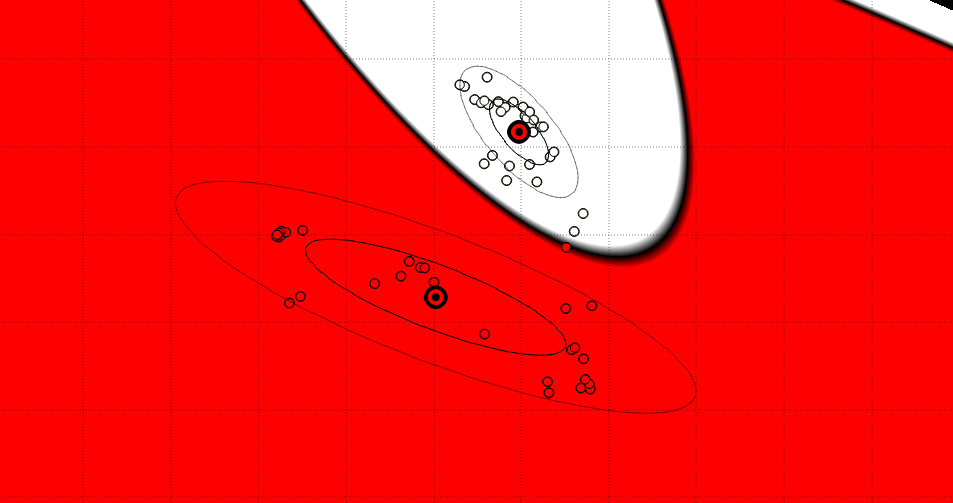
\includegraphics[height=0.11\textheight]{./classification/full_var_gmm_1_75pourcent_test.png}
	\caption{\bf Train ratio = 75\%}
    \end{subfigure}

\caption{GMM - Full covariance - 1 GMM per class}
\label{fig:train_ratio}
\end{figure}

As we have 60 samples in our dataset, with a training ratio of 10\%, only 6 samples are used for training. Thus, the trained model leads to bad performance. It's a case of under-fitting. However while increasing the training ratio, the model is able to correctly classify the data. Yet, with a too high training ratio, the model may over-fit on the data as we can see on figure \ref{fig:train_ratio_overfit} with a 10-fold. In fact, on training set, the variance is very low but on the testing set, the variance of the F1-measure is very high. Thus, it's a case of over-fitting. 

\begin{figure} [ht]
\centering
	\begin{subfigure}[h]{0.49\textwidth}
    \centering
	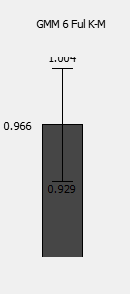
\includegraphics[height=0.14\textheight]{./classification/f_measure_testing_75pourcent.png}
	\caption{\bf F-measure on testing set}
	\end{subfigure}
    \begin{subfigure}[h]{0.49\textwidth}
    \centering
    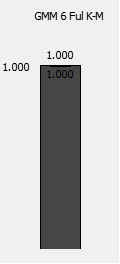
\includegraphics[height=0.14\textheight]{./classification/f_measure_training_75pourcent.png}
	\caption{\bf F-measure on training set}
    \end{subfigure}

\caption{GMM- Full covariance - 1 GMM per class - Train ratio = 75\%}
\label{fig:train_ratio_overfit}
\end{figure}

Thirdly, we have evaluated the effect of number component per class. We used a full-covariance matrix. We've seen previously in figure \ref{fig:train_ratio}, with one component per class, the model needs at least 50\% of training set. While increasing the number of component, the model gives better performances with less training data as we can see on figure \ref{fig:number_per_component}. In fact, with 2 components and a ratio of 25\%, the model gives bad classification. It needs 50\% of training set to correctly classify the data without over-fitting but it is more costly. With 5 components per class, the model needs 50\% less of training data to correctly classify the data but the model is over-fitting. In fact, the variance of the F-measure on testing set in this case is very high \ref{overfitting_case_5components} whereas on training set very low.

\begin{figure} [ht]
\centering
	\begin{subfigure}[h]{0.40\textwidth}
    \centering
	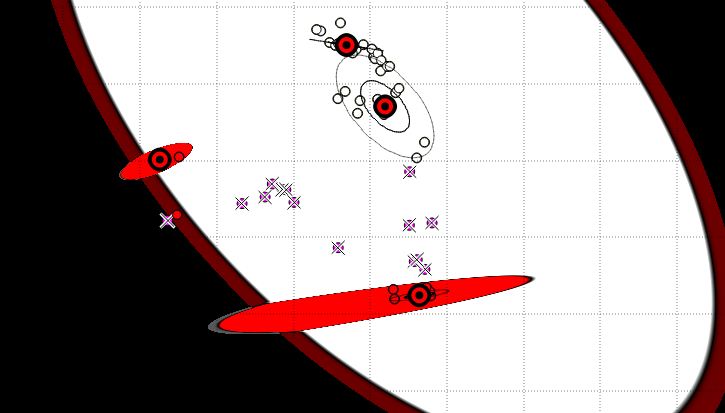
\includegraphics[height=0.12\textheight]{./classification/gmm_2_25pourcent_full_var.png}
	\caption{\bf 2 components per class - 25\% train ratio}
	\end{subfigure}
    \hspace{20mm}
	\begin{subfigure}[h]{0.40\textwidth}
    \centering
	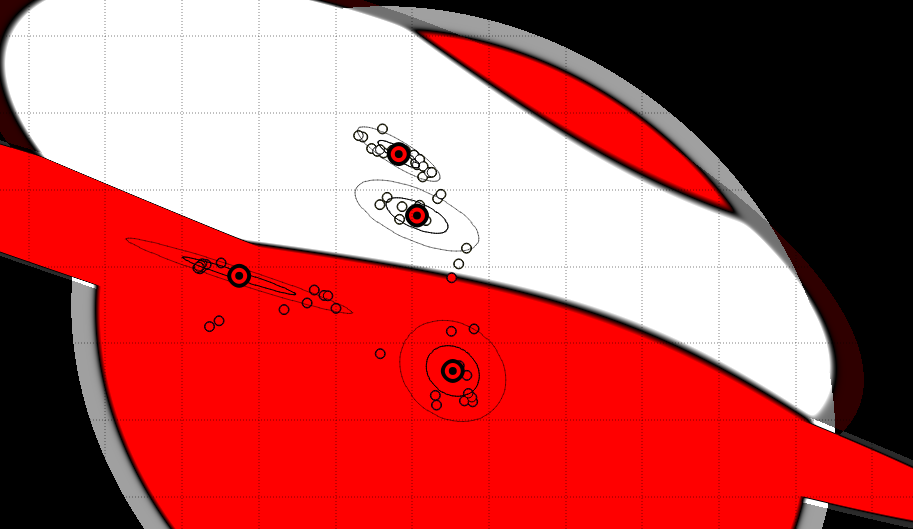
\includegraphics[height=0.12\textheight]{./classification/gmm_2_50pourcent_full_var.png}
	\caption{\bf 2 components per class - 50\% train ratio}
	\end{subfigure}\\
    \begin{subfigure}[h]{0.40\textwidth}
    \centering
    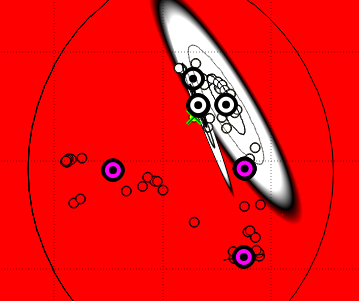
\includegraphics[height=0.12\textheight]{./classification/gmm_5_25pourcent_full_var.png}
	\caption{\bf 5 components per class - 25\% train ratio}
    \end{subfigure}
    \hspace{20mm}
    \begin{subfigure}[h]{0.40\textwidth}
    \centering
    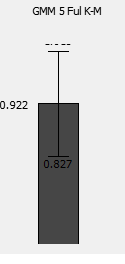
\includegraphics[height=0.12\textheight]{./classification/overfitting_case_gmm_5_25_.png}
	\caption{\bf F-measure on testing set - 25\% train ratio - 5 components}
    \label{overfitting_case_5components}
    \end{subfigure}

\caption{GMM - Full covariance}
\label{fig:number_per_component}
\end{figure}

Then, influence of covariance matrix is evaluated. We've seen previously that with a full covariance matrix and 2 components per class, we needs 50\% of training data. With a diagonal matrix and only 1 component per class, even if we used 100\% of training data, the model is not able to classify perfectly the data. But with 2 components per class and a training ratio of 33\%, the diagonal matrix model is able to perfectly classify the data without over-fitting. And for the spherical matrix, it needs 2 components but 50\% of training data. Results are shown in figure \ref{fig:covariance_influence}.


\begin{figure} [ht]
\centering
	\begin{subfigure}[h]{0.30\textwidth}
    \centering
	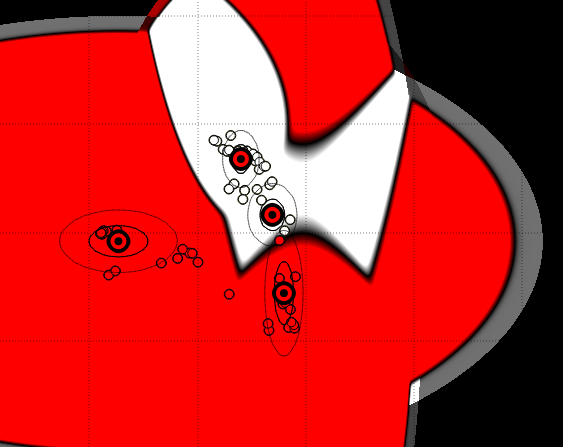
\includegraphics[height=0.13\textheight]{./classification/gmm_diag_cov_33pourcent_2gmm.png}
	\caption{\bf GMM Diagonal Covariance - 33\% - 2 Components}
	\end{subfigure}
    \hspace{3mm}
    \begin{subfigure}[h]{0.3\textwidth}
    \centering
    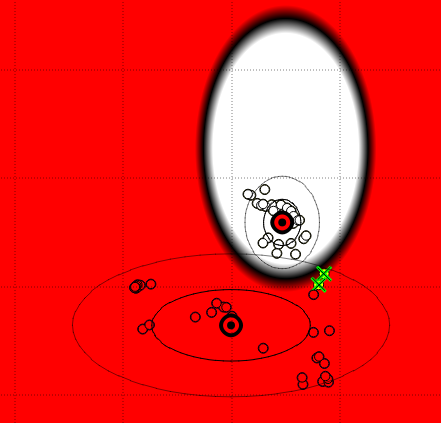
\includegraphics[height=0.13\textheight]{./classification/gmm_diag_cov_100pourcent_1gmm.png}
	\caption{\bf GMM Diagonal Covariance - 100\% - 1 Component}
    \end{subfigure}
    \hspace{3mm}
    \begin{subfigure}[h]{0.3\textwidth}
    \centering
    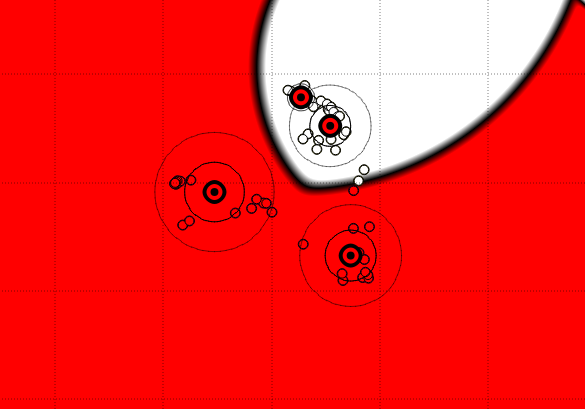
\includegraphics[height=0.13\textheight]{./classification/gmm_spherical_cov_50pourcent_2gmm.png}
	\caption{\bf GMM Spherical Covariance - 50\% - 2 Components}
    \end{subfigure}

\caption{Influence of covariance matrix}
\label{fig:covariance_influence}
\end{figure}



\subsection{SVM}
% Relié à la complexité dans l'algo d'optimisation
% C optimal : 10
% Faire apparaitre notion de sur apprentissage avec la comparaison des data point apartenant ou pas au training set
% But generalizable mais pas d'overfitting
%Describe method
%Explain the influence of support vectors in training step

In this section, we will consider two different Support Vector Machine algorithm. The first one performs linear classification and consist of one hyper-parameter which is C-Value. The second algorithm “RBF kernel” perform a non linear classification with one more hyper-parameter : the kernel width. The C-Value controls the influence of each individual support vector. A large C-Value will penalize the cost of misclassification dataset a lot. The best C-value is a trade-off between maximizing the margin and minimizing the classification errors. The kernel width defines the width of the kernel function. Large kernel width would imply a smoother fit and thus having a larger influence of neighborhood data point and vice-versa. 

\subsubsection{Linear}
As we can observe on figure \ref{fig:SVM_linear_C_value}, the resulting classification for different C-value and fixed train ratio (25\%). We note for the C-value : 0.5, there are 15 support vectors and 8 points misclassified. Then with higher C-value, we penalize the cost of misclassified data points in order to reduce them. The figure \ref{fig:SVM_linear_C_value_5} has still one misclassified points and 8 support vectors. The misclassified point is close to the other class, we can increase C-value and train ratio in order to reduce misclassified datapoints. Nevertheless, with a high C-value, the cost of misclassified datapoint will be high and the margin will reduce, thus forcing the algorithm to explain the data stricter and potentially overfit. The goal is to find a trade off between maximizing the margin and minimizing the classification errors. We can see an over-fitting case on figure \ref{fig:SVM_linear_C_value_1000}%(SVM_linear(c=1000,TR=50))
, which consist of only two support vectors and have a very low margin. Therefore, this model has a poor generalization.


\begin{figure}[ht]
\centering
\begin{subfigure}[h]{0.31\textwidth}
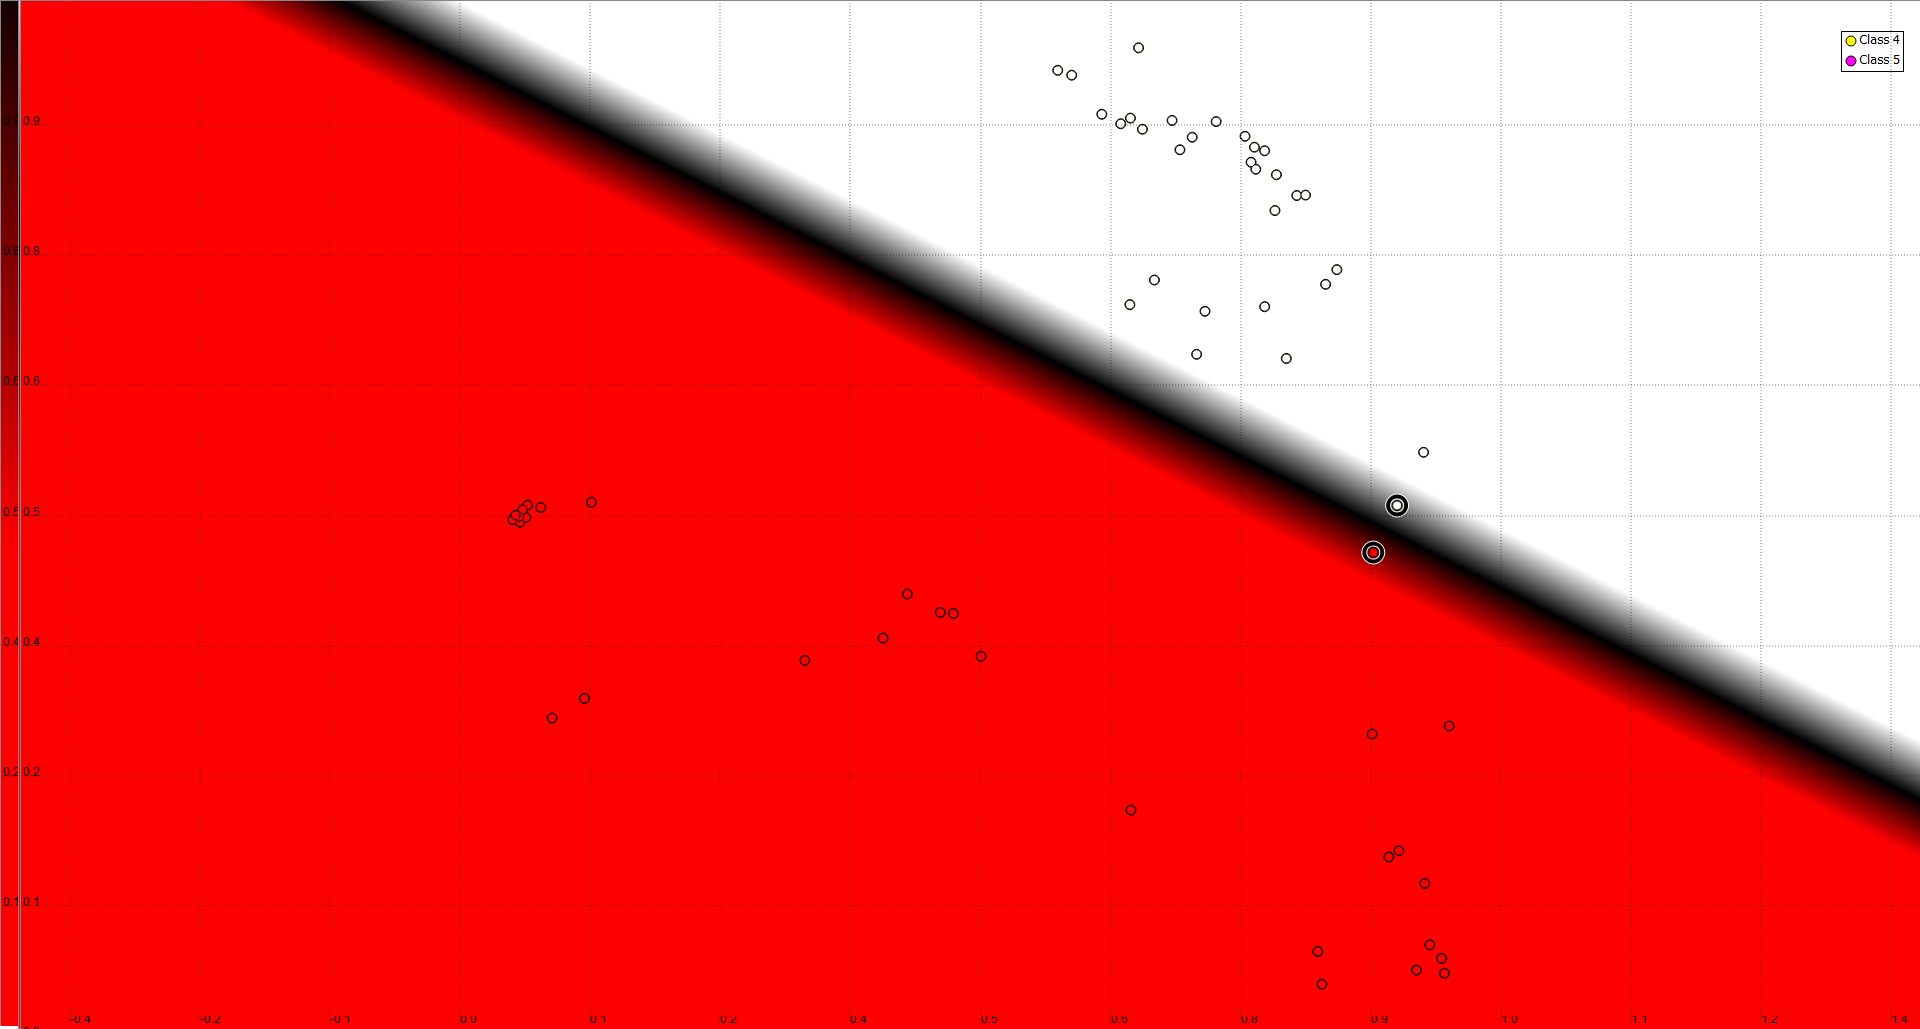
\includegraphics[height=0.11\textheight]{./classification/SVM_linear_c_1000_TR_50_.png}
\caption{\bf C-value : 1000 and train ratio : 50\%}
\label{fig:SVM_linear_C_value_1000}
\end{subfigure}
\hspace{20mm}
\begin{subfigure}[h]{0.31\textwidth}
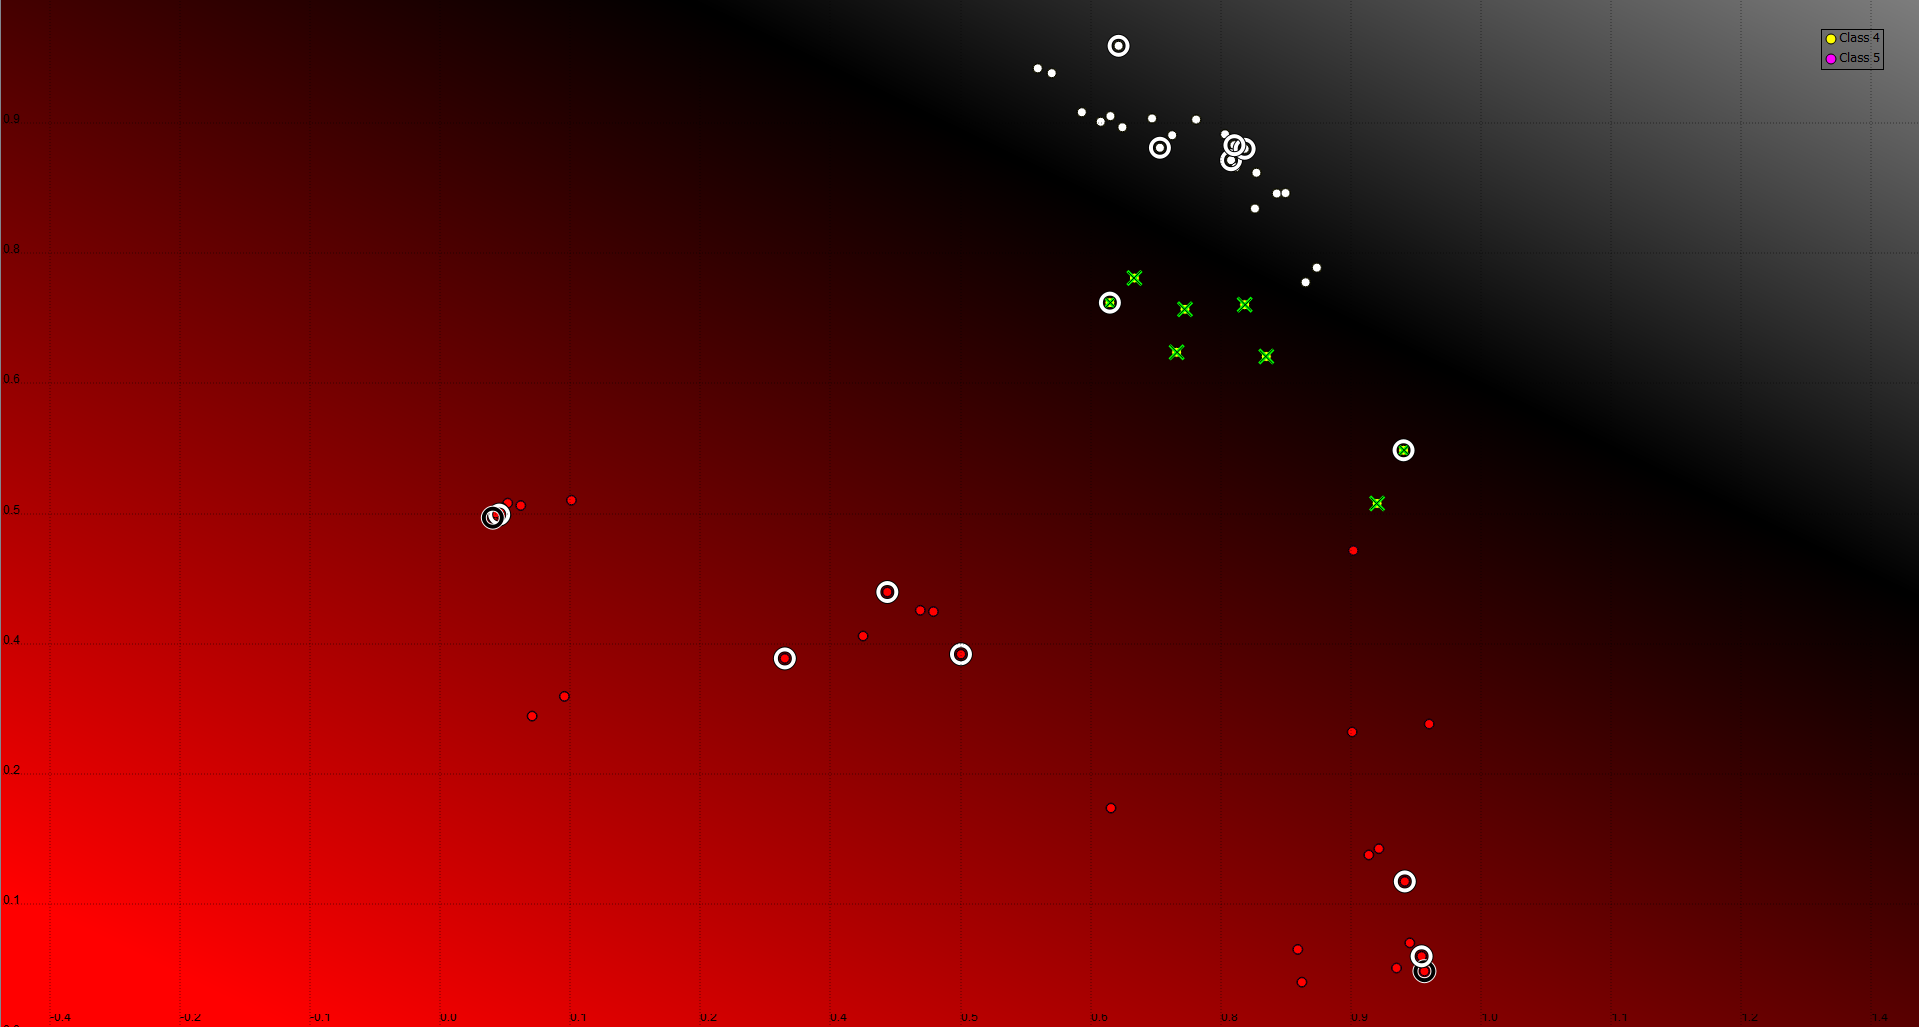
\includegraphics[height=0.11\textheight]{./classification/SVM_linear_c_0_5_TR_25_.png}
\caption{\bf C-value : 0.5 and train ratio : 25\%}
\end{subfigure}\\
\begin{subfigure}[h]{0.31\textwidth}
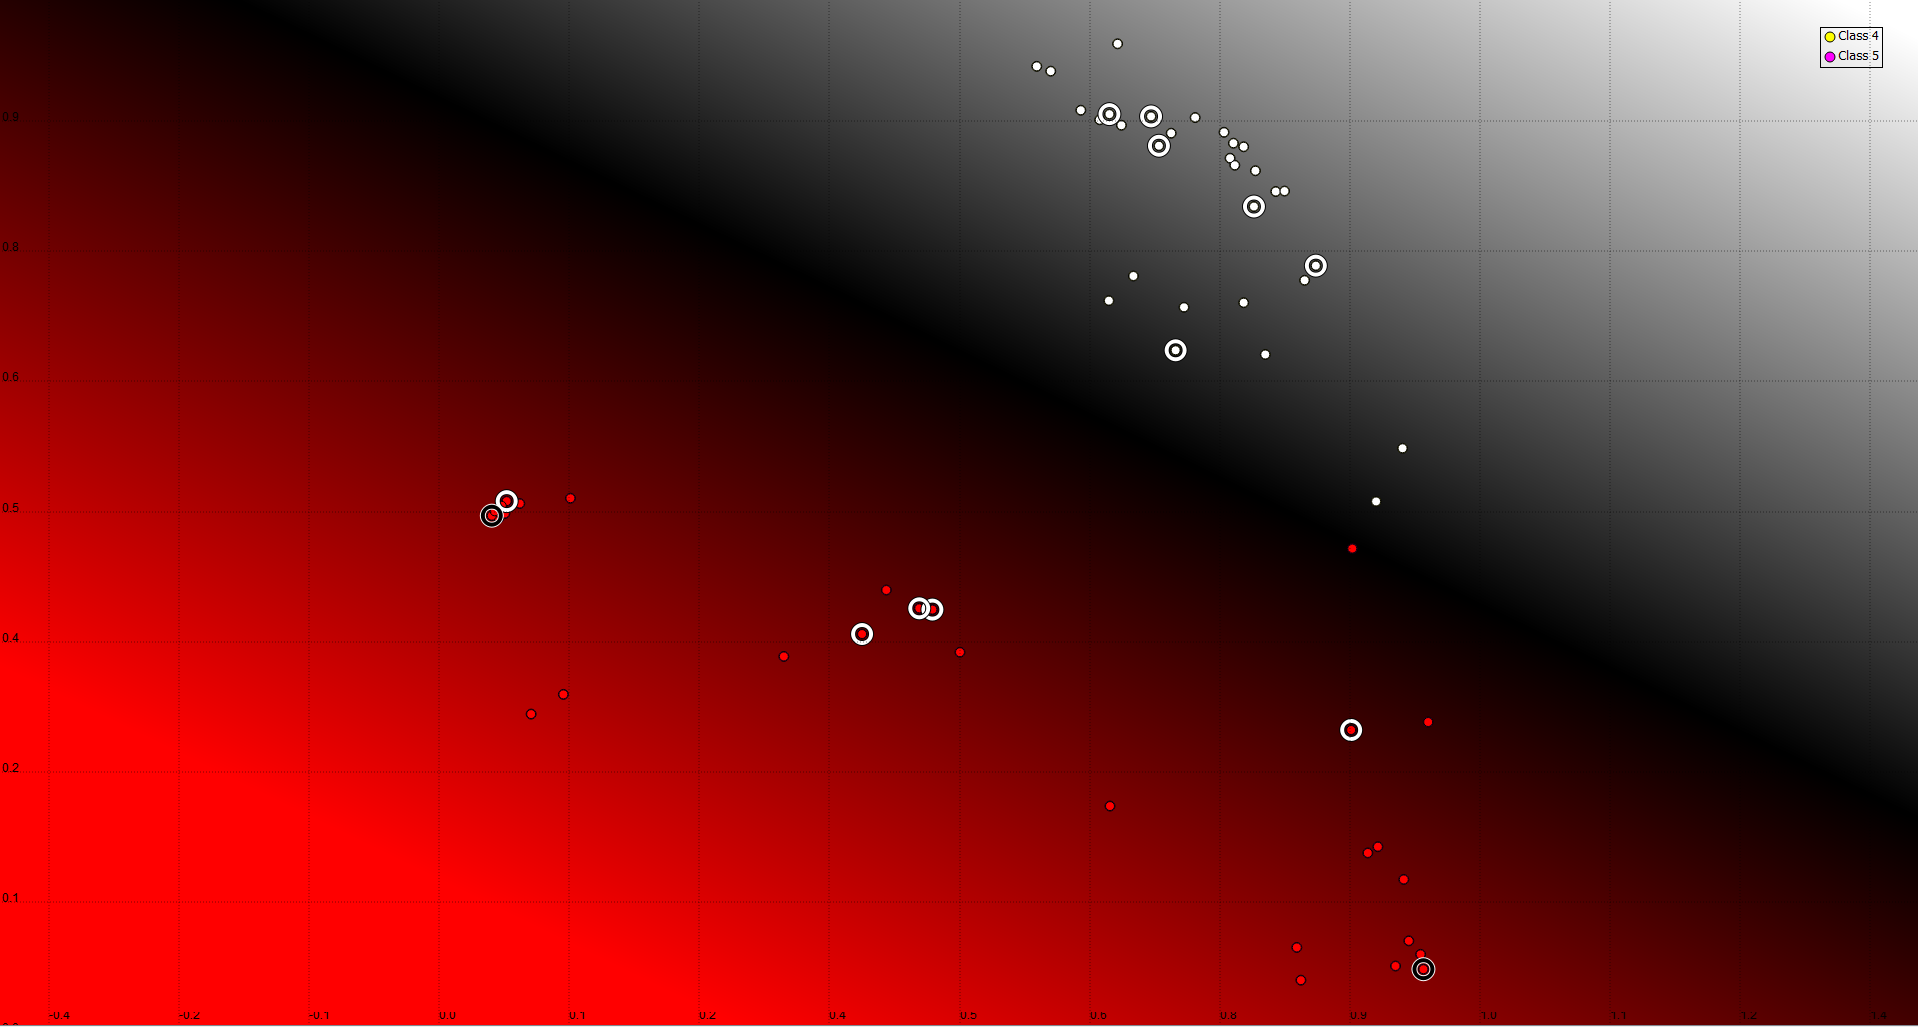
\includegraphics[height=0.11\textheight]{./classification/SVM_linear_c_1_TR_25_.png}
\caption{\bf C-value : 1 and train ratio : 25\%}
\end{subfigure}
\hspace{20mm}
\begin{subfigure}[h]{0.31\textwidth}
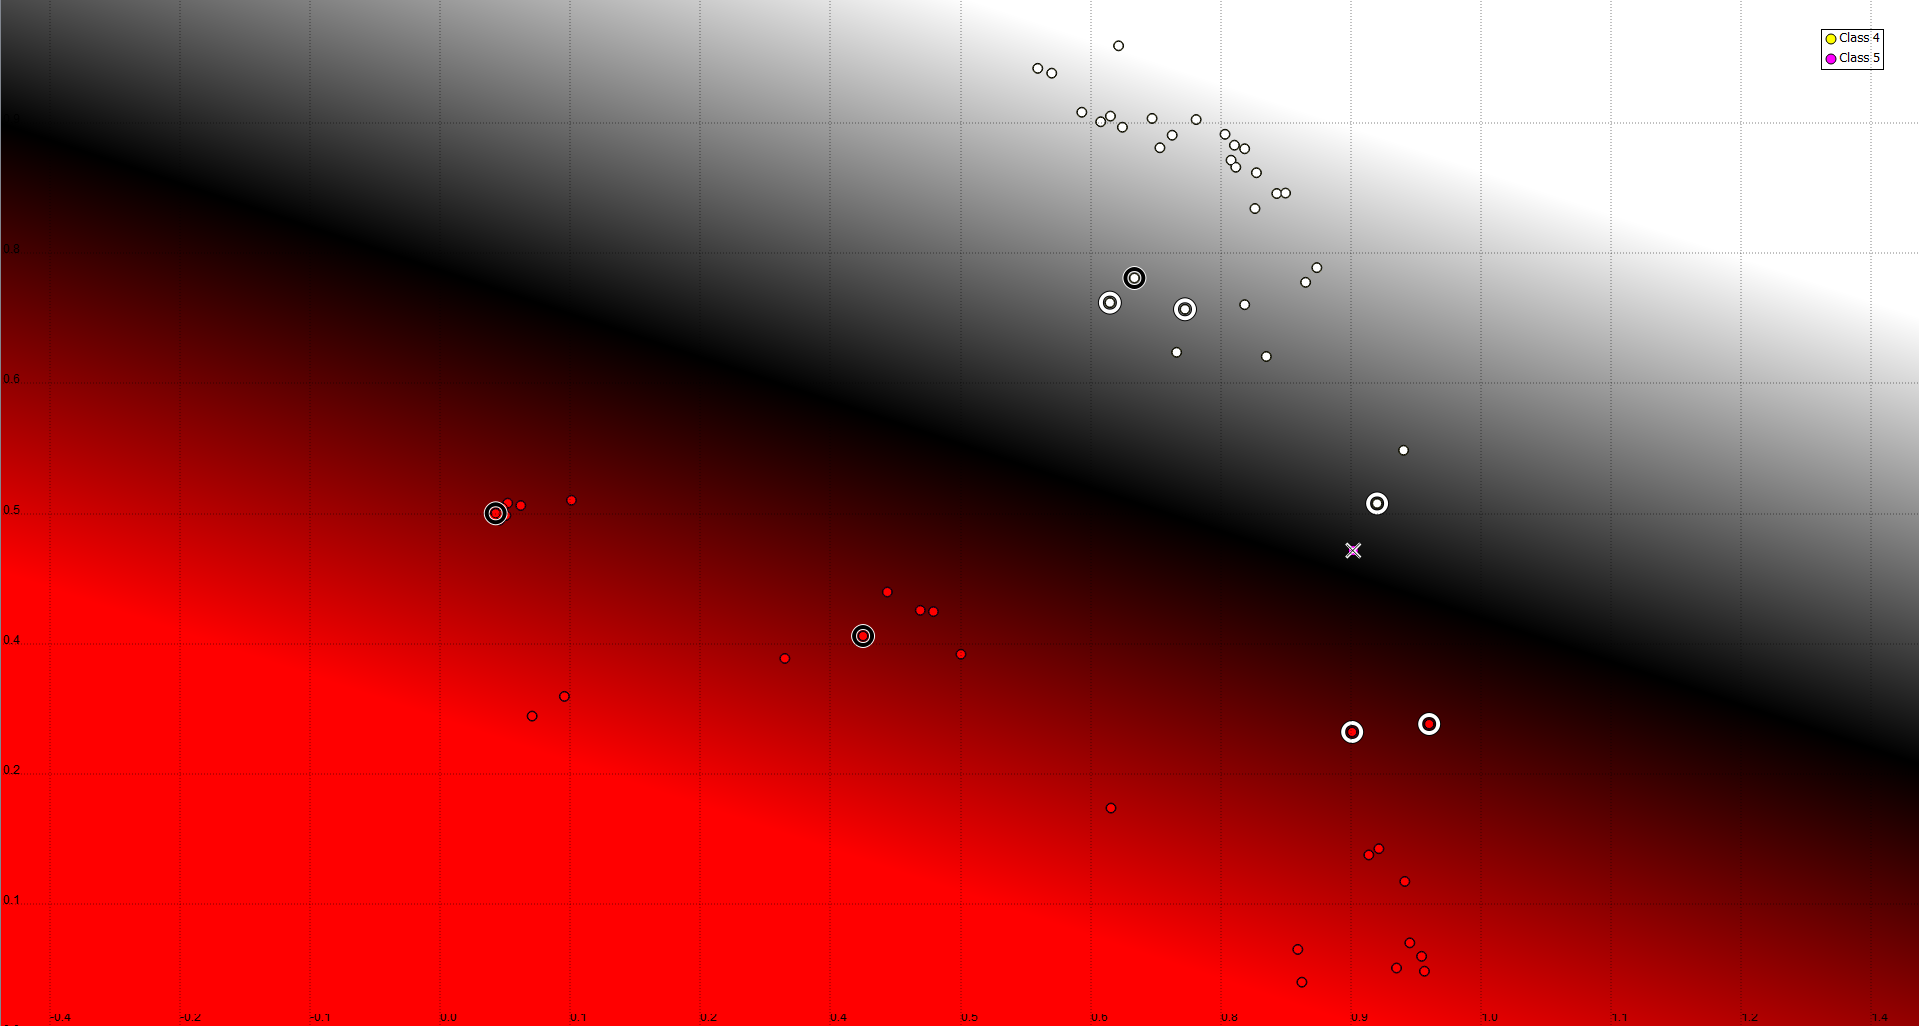
\includegraphics[height=0.11\textheight]{./classification/SVM_linear_c_5_TR_25_.png}
\caption{\bf C-value : 5 and train ratio : 25\%}
\label{fig:SVM_linear_C_value_5}
\end{subfigure}
\caption{SVM linear : influence of C-value}
\label{fig:SVM_linear_C_value}
\end{figure}

\subsubsection{RBF}

In our case, the dataset is linearly separable thus the linear SVM algorithm is sufficient. However, we perform RBF SVM algorithm to understand the influence of the hyper-parameters.

We observe on the figure \ref{fig:SVM_rbf_w_0_2_c_0_5_TR_25_} %SVM_rbf(w=0.2,c=0.5,TR=25).png
, the kernel width chosen is 0.2 and it seems to be the right size oh the kernel but we obtain 13 misclassified data points. This is due to the support vectors chosen by the algorithm. In order to perform a better model, we increase the C-Value to decrease the number of misclassified data points. On figure \ref{fig:SVM_rbf_w_0_2_c_1_TR_25_}
%SVM_rbf(w=0.2,c=1,TR=25)
, it has one misclassified data point, nevertheless the classification has a good generalization. If we continue to increase the C-Value, as we observe on figure \ref{fig:SVM_rbf_w_0_2_c_10_TR_25_}
%SVM_rbf(w=0.2,c=10,TR=25)
, the classification has none misclassified data point but it seems to overfit the dataset.
Finally, we try with a higher kernel width, as shown on figure \ref{fig:SVM_rbf_w_0_5_c_0_5_TR_25_}
%SVM_rbf(w=0.5,c=0.5,TR=25)
, the resulting classification has a good generalization and only one misclassified data point comparing to the figure \ref{fig:SVM_rbf_w_0_2_c_0_5_TR_25_}
%SVM_rbf(w=0.2,c=0.5,TR=25).png
, which has the same C-Value. Therefore, we can obtain better classification only by increasing the kernel width. 

\begin{figure}[!ht]
\centering
\begin{subfigure}[h]{0.31\textwidth}
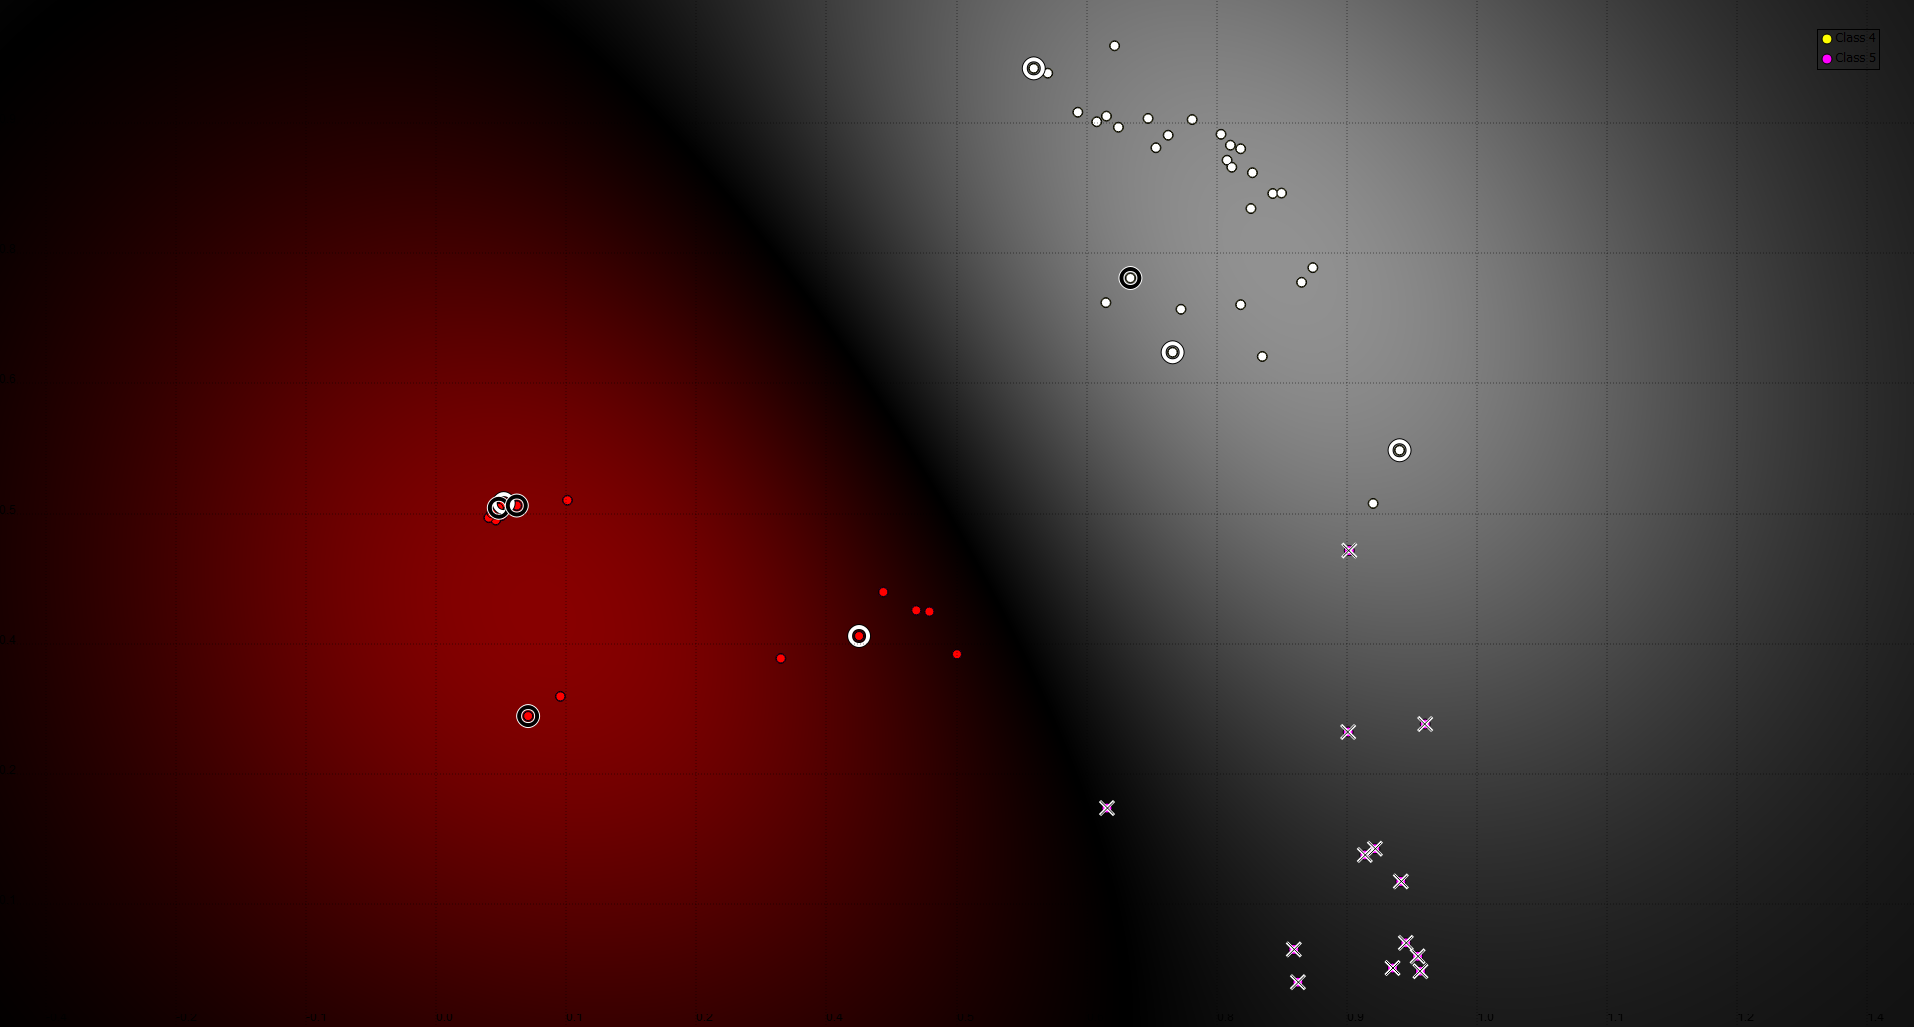
\includegraphics[height=0.11\textheight]{./classification/SVM_rbf_w_0_2_c_0_5_TR_25_.png}
\caption{\bf C-value : 0.5 and kernel width : 0.2}
\label{fig:SVM_rbf_w_0_2_c_0_5_TR_25_}
\end{subfigure}
\hspace{20mm}
\begin{subfigure}[h]{0.31\textwidth}
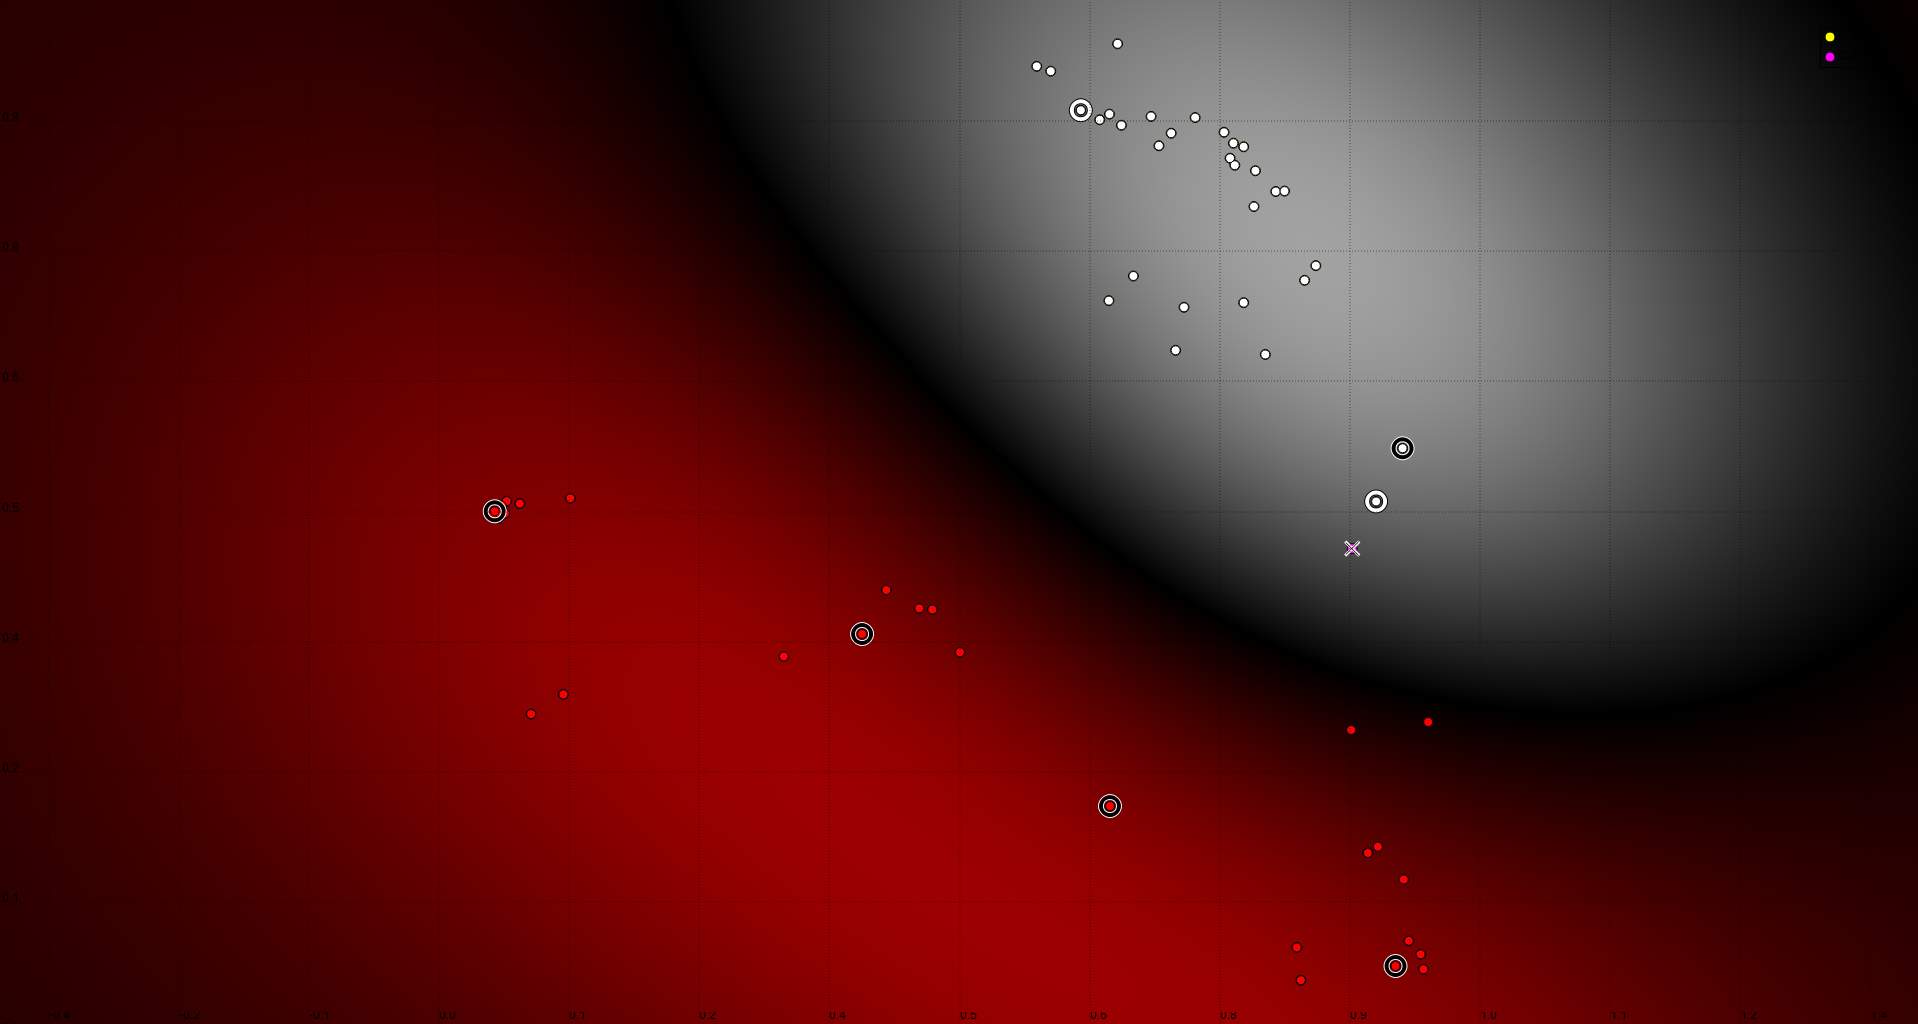
\includegraphics[height=0.11\textheight]{./classification/SVM_rbf_w_0_2_c_1_TR_25_.png}
\caption{\bf C-value : 1 and kernel width : 0.2}
\label{fig:SVM_rbf_w_0_2_c_1_TR_25_}
\end{subfigure}\\

\begin{subfigure}[h]{0.31\textwidth}
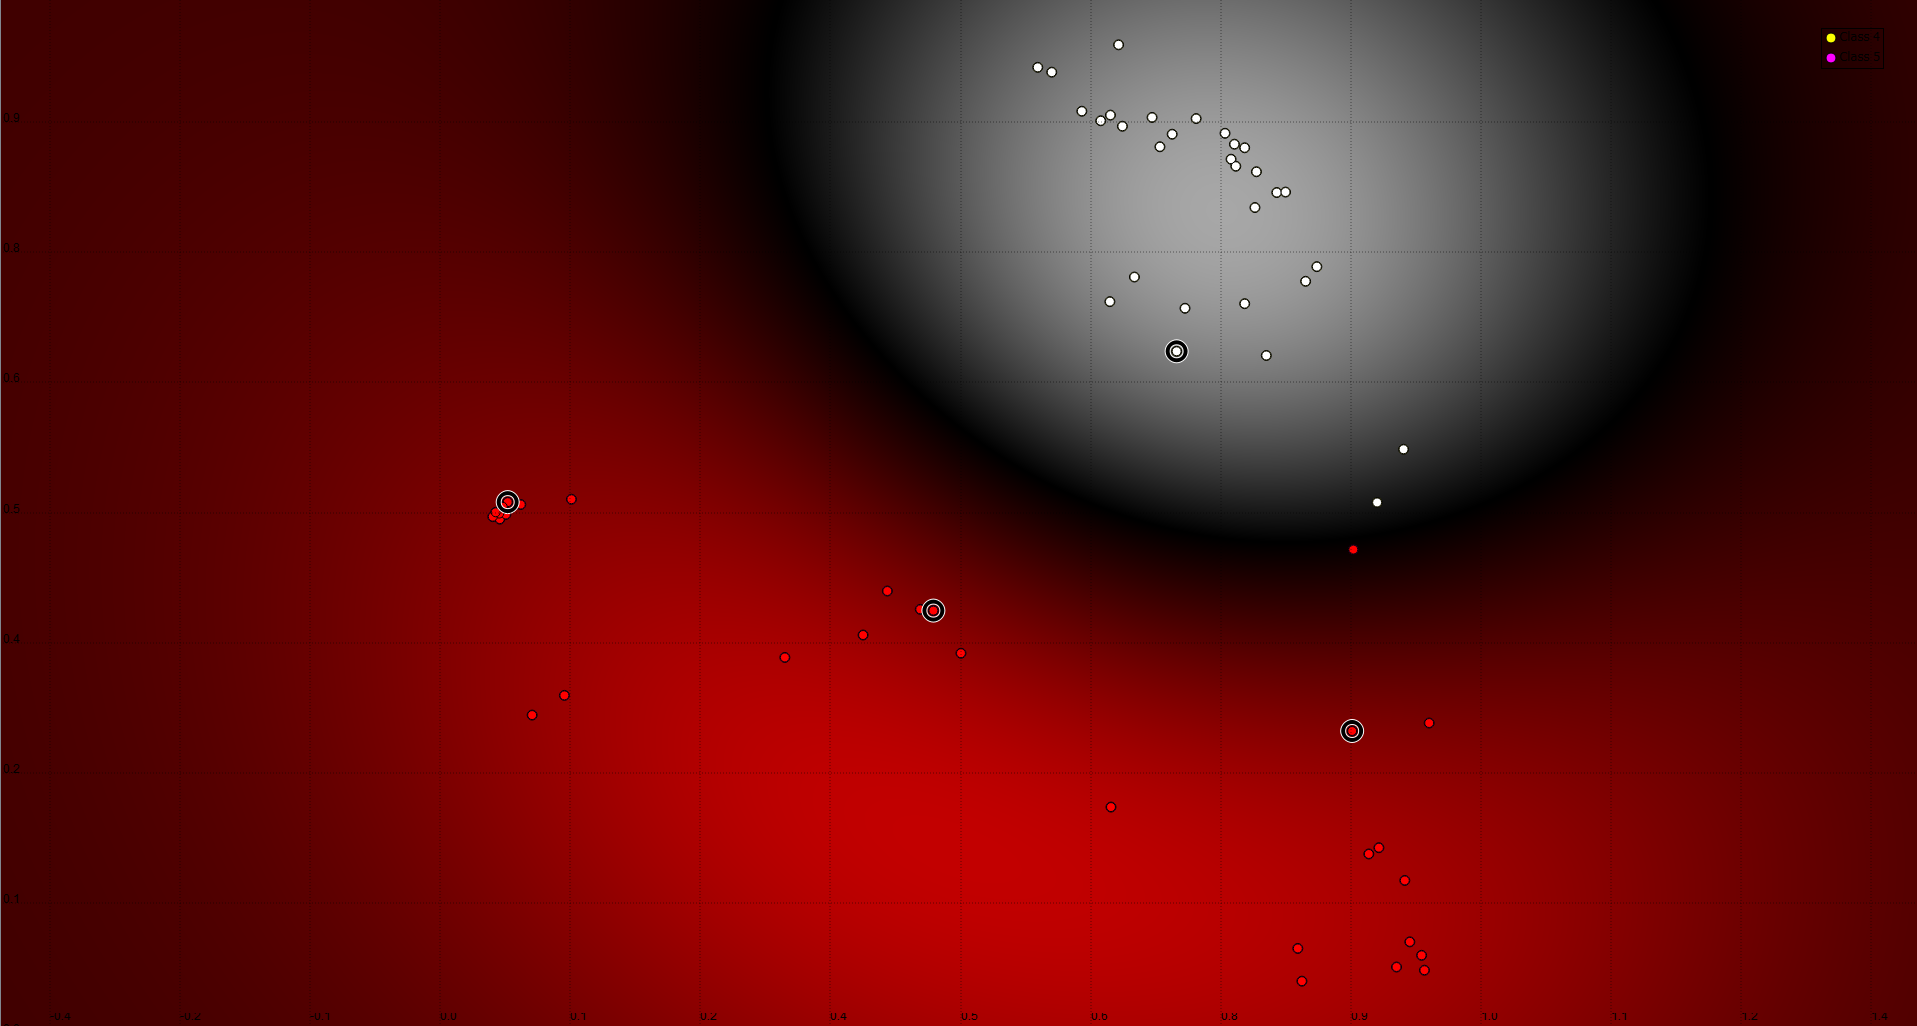
\includegraphics[height=0.11\textheight]{./classification/SVM_rbf_w_0_2_c_10_TR_25_.png}
\caption{\bf C-value : 10 and kernel width : 0.2}
\label{fig:SVM_rbf_w_0_2_c_10_TR_25_}
\end{subfigure}
\hspace{20mm}
\begin{subfigure}[h]{0.31\textwidth}
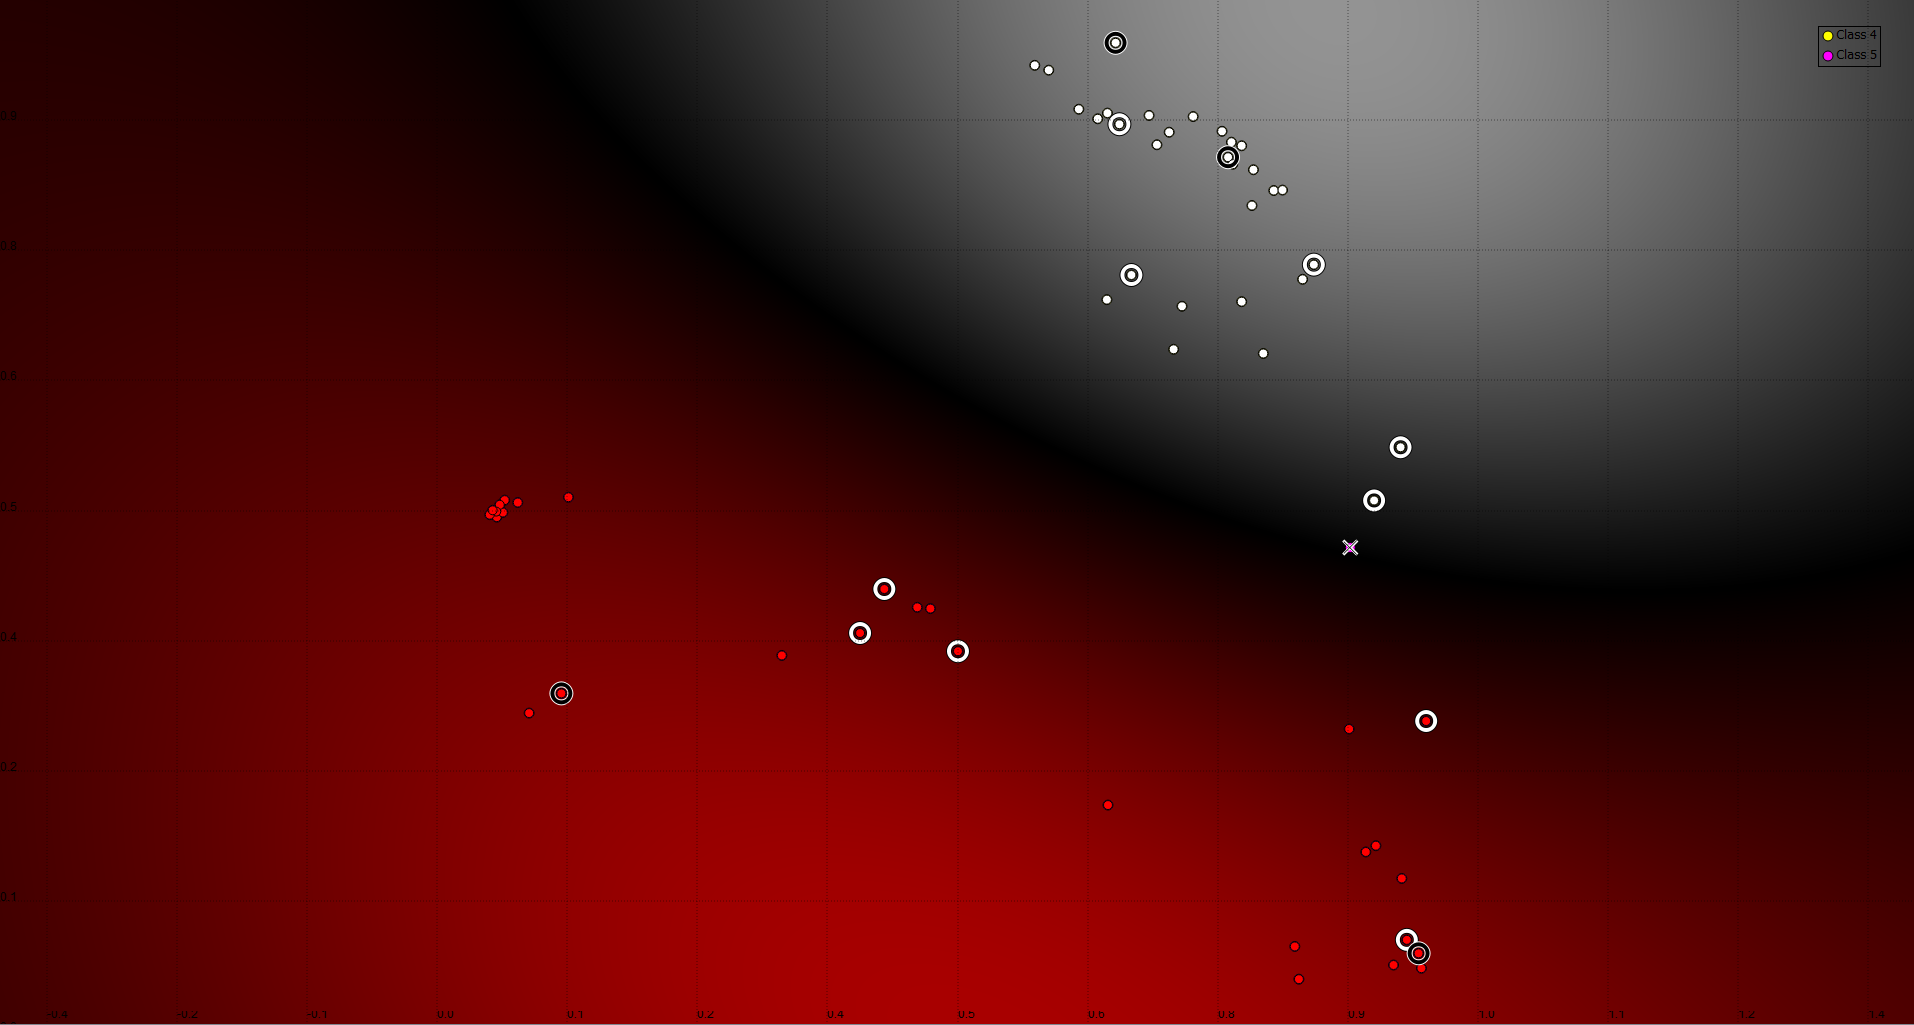
\includegraphics[height=0.11\textheight]{./classification/SVM_rbf_w_0_5_c_0_5_TR_25_.png}
\caption{\bf C-value : 0.5 and kernel width : 0.5}
\label{fig:SVM_rbf_w_0_5_c_0_5_TR_25_}
\end{subfigure}

\caption{SVM RBF : influence of kernel width and C-value}
\label{fig:SVM_RBF}
\end{figure}

%ADD F-measure



